\section{Approach Overview}
\label{sec:overview}

\begin{figure*}[t]
\begin{center}
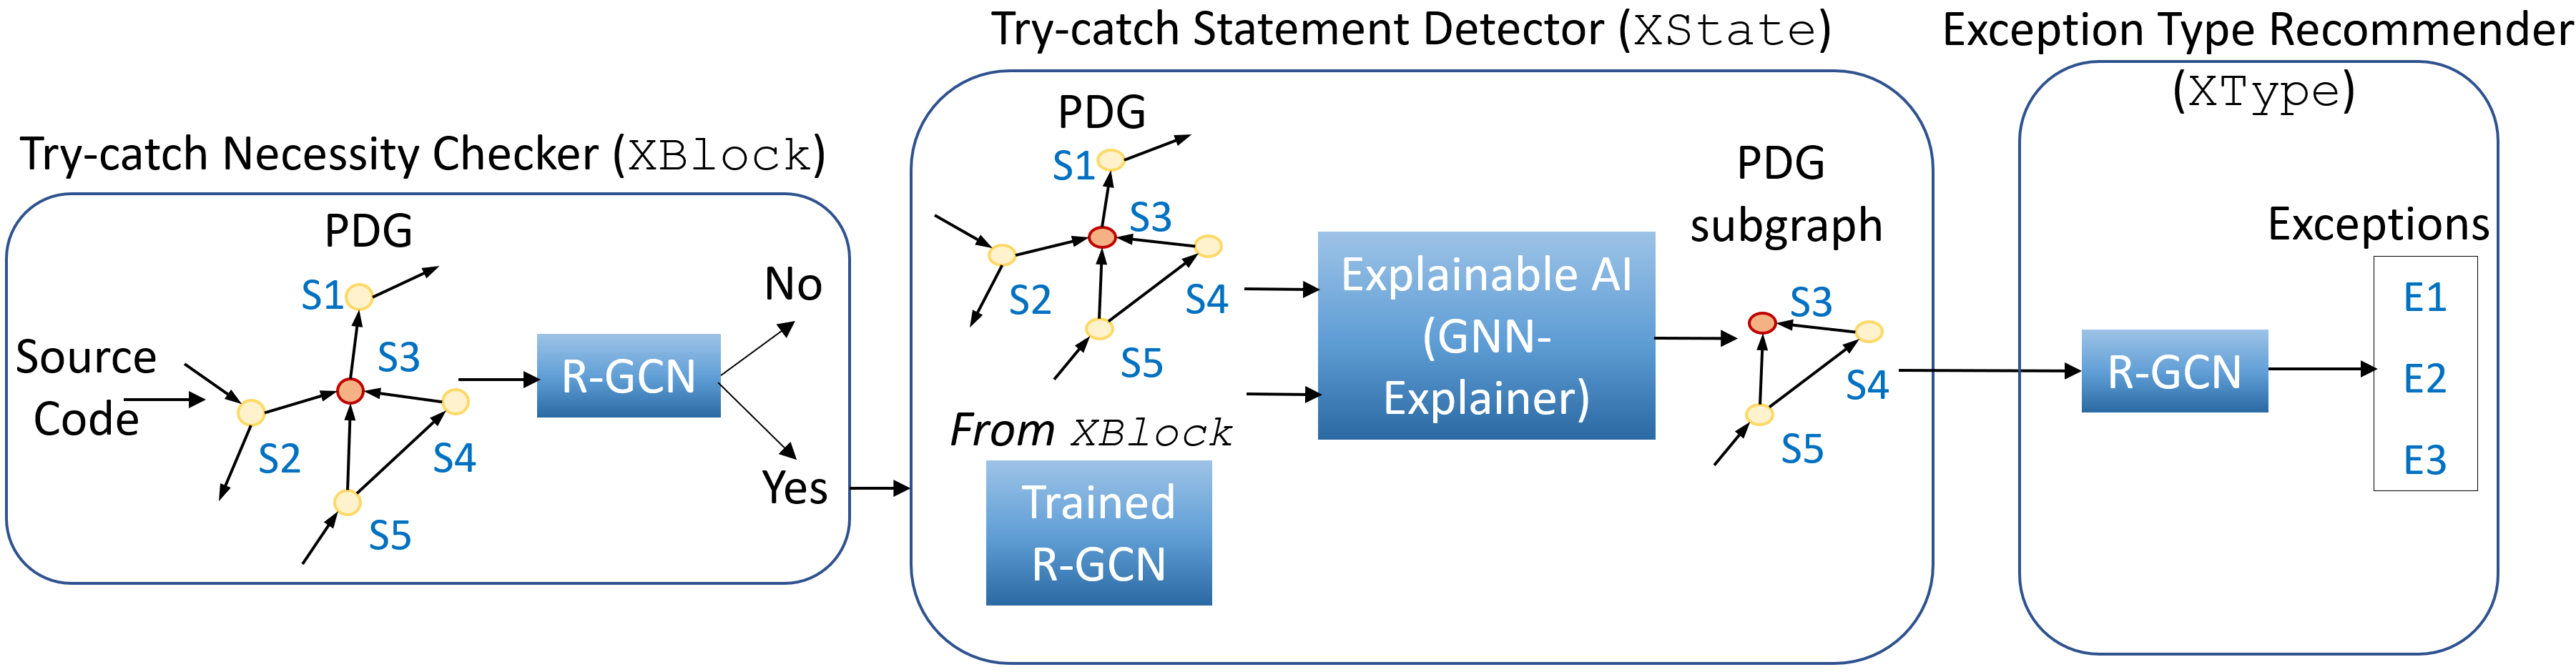
\includegraphics[width=5.4in]{overview-2.png}
\vspace{-10pt}
\caption{{\tool}: Architecture Overview}
\label{overview}
\end{center}
\end{figure*}

%Let us present the overview of our approach.

In general, {\tool} has three main components. The first
component, {\xblock}, aims to check if it is necessary to have a
\code{try-catch} block for a given code snippet $C$. We extract the
program dependence graph (PDG) from the source code using
DeepPDA~\cite{icse23} that is capable of generating the PDG for any
(in)complete code snippet. The PDG is used as an input for a
Relational Graph Convolutional Network (R-GCN)~\cite{rgcn}, which acts
as a classifier for {\xblock}. During training, we use the complete
source code in the open-source projects in which each positive sample
contains at least a \code{try-catch} block, and each negative sample
does not contain any. If there are multiple consecutive blocks, we
split them into individual ones. During prediction, {\xblock} uses the
trained R-GCN model to predict whether the code snippet $C$ needs a
\code{try-catch} block or not.

In the case that the code snippet $C$ needs a \code{try-catch} block,
the second component, {\xstate}, is aimed to detect which statements
in $C$ that need to be placed into a \code{try-catch} block.  We model
this task as an explanation task for {\xblock}. {\xstate} takes as
input: 1) the PDG of the given code snippet, and 2) the trained R-GCN
model for the \code{try-catch} necessity checker ({\xblock}), together
with the classification result ``Yes'' from that R-GCN model of
{\xblock}. {\xstate} leverages GNNExplainer~\cite{GNNExplainer}, a
graph-based, Explainable AI model to decide the statements in the PDG
that are most decisive and relevant to the reason why the code snippet
$C$ is required to have a \code{try-catch} block. During training, in
a positive sample, the statements in a \code{try-catch} block are
marked as positive, and the ones outside of the block as negative. All
the statements in a negative sample are marked as negative. During
prediction, the output of GNNExplainer is a list of statements in
$C$ (e.g., $S_3$, $S_4$, $S_5$) that made the R-GCN model in {\xblock}
to decide the need of a \code{try-catch} block. We consider them as
the statements to be in a \code{try-catch} block.

The third component is the exception type recommender, {\xtype}.
During training, the exception types in a \code{try-catch} block in
the positive samples are used as the labels. During prediction,
{\xtype} takes as input the result from GNNExplainer, which is the
subgraph of the PDG of the given source code $C$. Another R-GCN model
is used and acted as a classifier for all the exception
types.
